% ==========================================
% BAB I PENDAHULUAN
% ==========================================
\chapter{PENDAHULUAN}
\label{chap:pendahuluan}
% --- Latar Belakang ---
\section{Latar Belakang}
Kolaborasi merupakan salah satu keterampilan paling penting bagi mahasiswa di era pendidikan tinggi modern. Perubahan pola pembelajaran yang semakin berbasis proyek dan aktivitas lintas disiplin menuntut mahasiswa untuk mampu bekerja sama secara efektif dengan individu yang memiliki latar belakang, minat, dan keterampilan yang beragam. Menurut \textcite{laalBenefitsCollaborativeLearning2012a}, kolaborasi tidak hanya meningkatkan pencapaian akademik, tetapi juga memperkuat kompetensi sosial, komunikasi, dan pemecahan masalah. Dalam konteks dunia kerja yang semakin kompetitif, pengalaman kolaboratif selama masa studi menjadi fondasi penting bagi kesiapan profesional mahasiswa.

Meskipun kolaborasi menjadi kebutuhan yang semakin besar, proses menemukan rekan kolaborasi yang sesuai bukanlah hal yang mudah. Mahasiswa umumnya menemukan partner melalui pendekatan informal seperti rekomendasi teman, relasi kelas, atau grup percakapan daring. Pola ini membuat akses terhadap calon partner menjadi sangat bergantung pada ukuran dan kualitas jaringan sosial individu. \Textcite{granovetterStrengthWeakTies1983} berpendapat bahwa jaringan informal dapat bersifat terbatas dan tidak merata, sehingga individu dengan jaringan kecil berpotensi kehilangan akses terhadap peluang sosial yang bernilai. Dalam konteks mahasiswa, hal ini menyebabkan banyak peluang kolaboratif terlewat karena informasi tidak terdistribusi secara terbuka kepada seluruh mahasiswa.

Selain tantangan akses, persoalan yang lebih mendasar adalah kesulitan mahasiswa dalam menilai kecocokan antar individu. Kerja tim yang efektif tidak hanya ditentukan oleh minat yang sama, tetapi juga oleh keselarasan keterampilan, pengalaman, preferensi gaya kerja, serta pola komunikasi. \textcite{mathieuTeamEffectiveness199720072008} menunjukkan bahwa kecocokan komposisi tim sangat berpengaruh terhadap efektivitas kolaborasi, terutama dalam proyek yang menuntut kreativitas dan koordinasi intensif. Namun, mahasiswa sering kali tidak memiliki data yang cukup mengenai atribut-atribut tersebut dari calon partner, sehingga keputusan memilih partner dilakukan secara intuitif tanpa dasar informasi yang kuat.

Ketidaksesuaian dalam memilih rekan juga dapat menimbulkan berbagai masalah dalam dinamika tim. Ketidaksesuaian gaya kerja antar anggota tim dapat meningkatkan konflik, menurunkan kinerja, dan memperpanjang waktu adaptasi tim. Hal ini sejalan dengan temuan \textcite{ensherEffectsPerceivedDiscrimination2001} bahwa keselarasan kompetensi dan ekspektasi merupakan faktor penting dalam keberhasilan kolaborasi jangka pendek maupun jangka panjang. Tanpa pemetaan kecocokan yang jelas sejak awal, tim mahasiswa berisiko menghadapi friksi internal yang menghambat capaian akademik maupun performa kompetisi.

Di sisi lain, platform digital yang tersedia saat ini belum sepenuhnya menjawab kebutuhan pencarian partner bagi mahasiswa. Sebagian besar platform seperti LinkedIn, Glints, atau Kalibrr dirancang untuk kebutuhan profesional dan rekrutmen formal, bukan untuk konteks pembentukan tim mahasiswa. Platform tersebut tidak menyediakan mekanisme rekomendasi berbasis keselarasan minat, keterampilan, preferensi kerja, atau pengalaman kolaborasi mahasiswa. Sistem rekomendasi yang mempertimbangkan atribut multidimensi dapat meningkatkan efisiensi proses pembentukan tim secara signifikan. Ketiadaan platform yang secara khusus memfasilitasi pencarian rekan kolaborasi membuat mahasiswa sering kali mengandalkan proses \textit{trial-and-error} dalam menentukan partner. Proses ini tidak hanya memakan waktu, tetapi juga dapat menyebabkan pembentukan tim yang tidak optimal. 


% \item	Kondisi atau situasi topik yang dibahas beserta permasalahannya, misalnya tentang pengelolaan informasi di puskesmas daerah pedesaan dan masalah yang dihadapi.
% \item	Berbagai solusi yang teDlah diterapkan atau solusi yang tersedia dan memungkinkan untuk diterapkan untuk menyelesaikan masalah tersebut.
% \end{enumerate}

% --- Rumusan Masalah ---
% \section{Rumusan Masalah}
% Rumusan Masalah berisi masalah utama yang dibahas dalam tugas akhir. Rumusan masalah yang baik memiliki struktur sebagai berikut:
% \begin{enumerate}
% \item	Pokok persoalan dari kondisi atau situasi yang ada saat ini. Dengan kata lain, jelaskan kelemahan atau kekurangan dari kondisi, situasi, atau solusi yang dijelaskan pada latar belakang. Ini merupakan pokok rumusan masalah.
% \item	Elaborasi lebih lanjut urgensi penyelesaian masalah tersebut (mengapa penting untuk diselesaikan dan akibat yang dapat terjadi jika tidak diselesaikan).
% \item	Usulan singkat terkait dengan solusi yang ditawarkan untuk menyelesaikan persoalan.
% Penting untuk diperhatikan bahwa persoalan yang dideskripsikan pada subbab ini akan dipertanggungjawabkan di bab Evaluasi (apakah terselesaikan atau tidak).
% \end{enumerate}
\section{Rumusan Masalah}
Berdasarkan Latar Belakang di atas, maka rumusan masalah dari tugas akhir ini adalah bagaimana mengembangkan sistem yang dapat membantu mahasiswa menemukan dan memilih rekan kolaborasi yang sesuai dengan minat, keterampilan, dan preferensi kerja mereka secara lebih terarah dan relevan.


% --- Tujuan ---
\section{Tujuan}
% Tuliskan tujuan utama dan/atau tujuan detail yang akan dicapai dalam pelaksanaan tugas akhir. Fokuskan pada hasil akhir yang ingin diperoleh setelah tugas akhir diselesaikan, terkait dengan penyelesaian persoalan pada rumusan masalah. Penting untuk diperhatikan bahwa tujuan yang dideskripsikan pada subbab ini akan dipertanggungjawabkan di akhir pelaksanaan tugas akhir apakah tercapai atau tidak. Tuliskan kriteria keberhasilan tugas akhir ini.
Tujuan dari tugas akhir ini adalah mengembangkan sistem yang dapat membantu mahasiswa dalam menemukan dan memilih rekan kolaborasi yang sesuai dengan minat, keterampilan, dan preferensi kerja mereka.


% --- Batasan Masalah ---
\section{Batasan Masalah}
% Tuliskan batasan-batasan yang diambil dalam pelaksanaan tugas akhir. Batasan ini dapat dihindari (bersifat opsional, tidak perlu ada) jika topik atau judul tugas akhir dibuat cukup spesifik.
Batasan masalah dari tugas akhir ini adalah sebagai berikut.
\begin{enumerate}
    \item Sistem difokuskan untuk kebutuhan mahasiswa sebagai pengguna utama, khususnya dalam konteks pencarian rekan kolaborasi (\textit{people-to-people}) pada kegiatan akademik maupun non-akademik.
    \item Profil mahasiswa yang digunakan dalam proses rekomendasi dibatasi pada aspek-aspek tertentu, meliputi minat, keterampilan yang dikuasai, pengalaman relevan, preferensi gaya kerja, serta parameter lain yang mendukung penilaian kecocokan antar mahasiswa.
\end{enumerate}

% --- Metodologi Pengerjaan TA ---
% \section{Metodologi}
% Tuliskan semua tahapan yang akan dilalui selama pelaksanaan tugas akhir. Tahapan ini spesifik untuk menyelesaikan persoalan tugas akhir. Khusus untuk penyusunan proposal ini, jelaskan secara detail:
% \begin{enumerate}
% \item	Tahapan investigasi pengumpulan fakta di latar belakang untuk merumuskan masalah.
% \item	Langkah-langkah pencarian, pengelompokan, dan penapisan literatur atau sumber informasi untuk mengumpulkan informasi yang relevan tentang topik yang diangkat, termasuk teori (konsep atau teori apa saja yang perlu dicari), hal-hal yang telah dicapai oleh orang lain (cara mencari dan kata kuncinya), dan berbagai informasi pendukung, untuk mencari solusi terhadap masalah yang dibahas. Gunakan metodologi yang tepat dalam menggali informasi dan dokumentasikan prosesnya (termasuk rekaman wawancara atau survei) di dalam Lampiran, termasuk tautan ke video atau foto. Hasil penggalian informasi ini akan dijelaskan secara sistematis di Bab II Studi Literatur.
% \end{enumerate}
\section{Metodologi}
Tugas akhir ini menggunakan model \textit{Software Development Life Cycle} (SDLC) \textit{Waterfall}, sebagaimana dijelaskan oleh Ian Sommerville dalam Software Engineering (10th ed.). Model \textit{Waterfall} dipilih karena memberikan alur kerja yang terstruktur, terdokumentasi, dan linear, sehingga sesuai untuk proyek Tugas Akhir ini yang memerlukan pemisahan modul antar anggota kelompok, namun tetap harus terintegrasi pada tahap akhir.
Selain itu, proses \textit{design and evaluation} pada tahap \textit{Waterfall} menggunakan pendekatan textit{User-Centered Design} (UCD – ISO 9241-210) untuk memastikan platform kolaborasi mahasiswa benar-benar sesuai kebutuhan pengguna. Alur SDLC yang digunakan pada pengerjaan tugas akhir ini dapat dilihat pada Gambar \ref{gambar:sdlc}.

\begin{figure}[h] % pilihan opsi yang disarankan: t = top, b = bottom, h = here
	\centering
  \captionsetup{justification=centering}
    	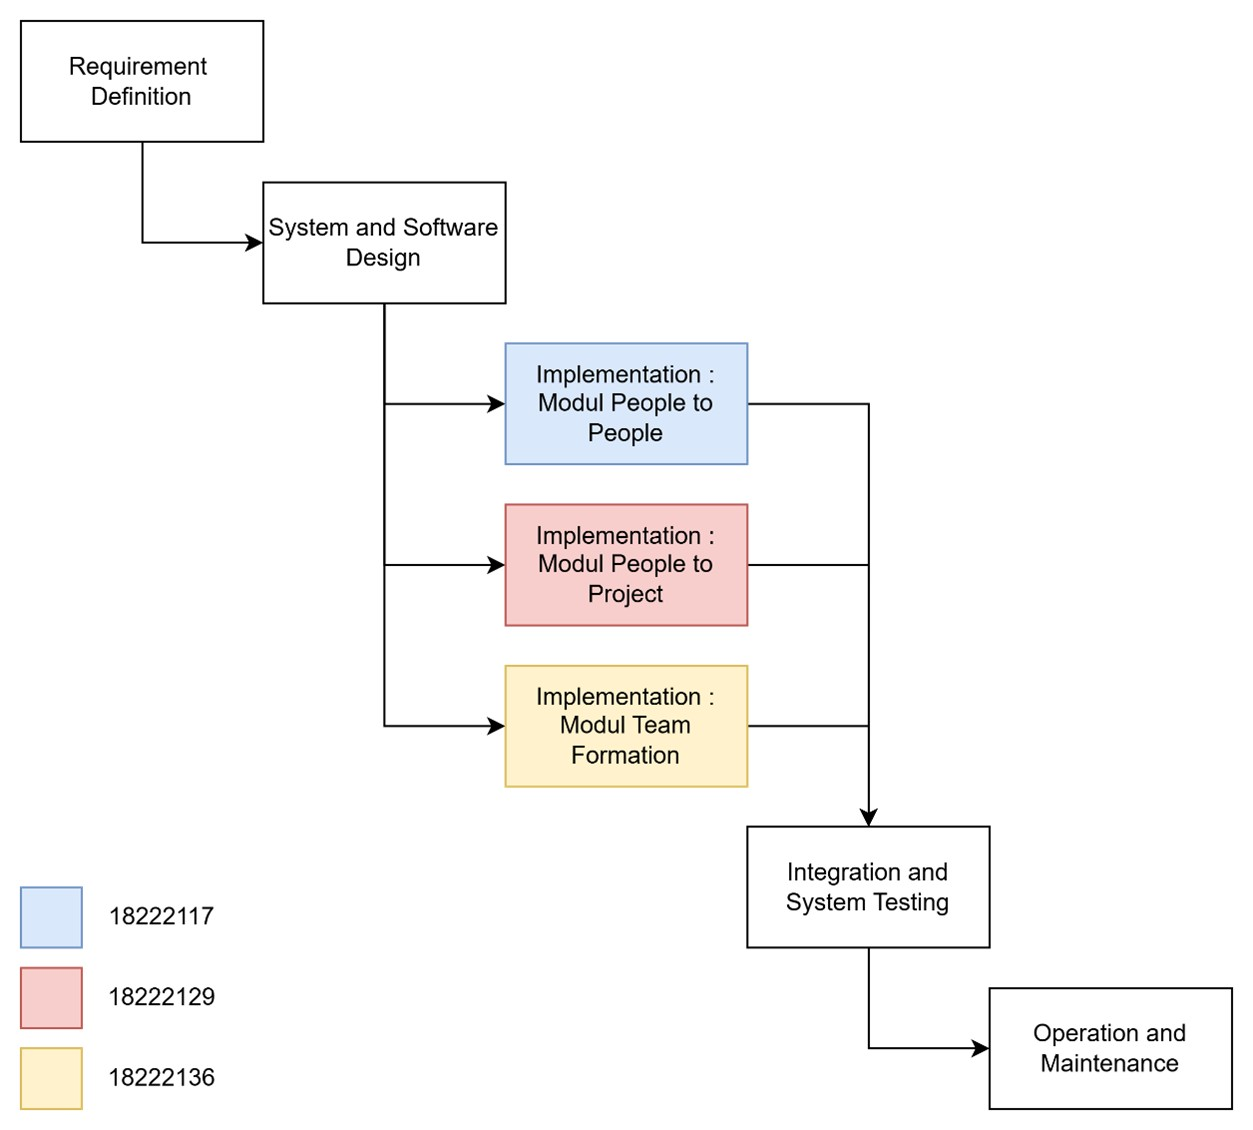
\includegraphics[width=0.65\textwidth]{image/SDLC.jpg}
	\caption{Contoh model SDLC \textit{Waterfall}}
	\label{gambar:sdlc}
\end{figure}

Berikut merupakan penjelasan detail untuk masing – masing fase.
\begin{enumerate}
\item \textit{Requirement Definition}

Pada tahap ini dilakukan proses pengumpulan dan analisis kebutuhan pengguna dan sistem. Kegiatan meliputi penyebaran survei dan observasi terkait pengalaman mahasiswa dalam mencari tim dan menentukan peran. Data ini digunakan untuk mengidentifikasi masalah utama dalam proses pembentukan tim, keterbatasan akses informasi, serta kesulitan menentukan role yang tepat. Seluruh temuan kemudian dirumuskan dalam bentuk kebutuhan fungsional dan non-fungsional, yang disusun ke dalam dokumen \textit{Software Requirement Specification} (SRS) sebagai fondasi seluruh tahap berikutnya.

\item \textit{System and Software Design}

Tahap ini menghasilkan rancangan sistem secara menyeluruh, mulai dari arsitektur perangkat lunak, diagram UML, hingga desain antarmuka. Prinsip \textit{User-Centered Design} (UCD) digunakan untuk memastikan rancangan fitur sesuai dengan kebutuhan pengguna nyata berdasarkan temuan pada tahap sebelumnya. Fase ini mencakup penyusunan use case, flow diagram, class diagram, serta prototipe wireframe untuk modul \textit{People-to-People, People-to-Project, dan Team Formation}. Pada tahap ini juga dirancang logika \textit{Affinity-Based Role Recommendation}, yaitu kerangka rekomendasi role berdasarkan kompatibilitas peran dan preferensi kontribusi mahasiswa.

\item \textit{Implementation and Unit Testing}

Implementasi sistem dilakukan berdasarkan desain yang telah disepakati. Pada proyek ini, setiap anggota kelompok bertanggung jawab untuk mengembangkan satu modul berbeda, yaitu modul \textit{People-to-People Matching} (Ahmad Fawwazi, 18222117), modul \textit{People-to-Project Matching} (Muhammad Faishal Putra, 18222129) dan modul \textit{Team Formation} (Muhammad Faishal Firdaus, 18222136). Setiap modul dikembangkan secara independen namun tetap mengikuti standar desain yang sama agar mudah diintegrasikan. Setelah implementasi tiap modul selesai, dilakukan \textit{unit testing} untuk memastikan setiap fungsi berjalan sesuai spesifikasi tanpa adanya kesalahan logika dasar.

\item \textit{Integration and System Testing}

Tahap ini menggabungkan ketiga modul menjadi satu platform yang utuh. Proses integrasi mencakup penyatuan alur data, sinkronisasi API atau fungsi internal, serta penyamaan format keluaran, terutama antara modul rekomendasi role dan modul pembentukan tim. Setelah sistem terintegrasi, dilakukan system testing mencakup pengujian fungsional, kompatibilitas alur, dan performa. Sebagai bagian dari prinsip UCD, dilakukan pula usability testing yang menilai kemudahan penggunaan platform oleh mahasiswa sebagai target pengguna. Evaluasi ini menjadi dasar penyempurnaan sistem sebelum memasuki tahap operasional.

\item \textit{Operation and Maintenance}

Tahap akhir dalam model Waterfall mencakup proses pemeliharaan sistem setelah pengujian. Kegiatan dalam fase ini meliputi perbaikan bug, penyempurnaan alur interaksi, serta pengoptimalan fitur berdasarkan umpan balik dari proses \textit{usability testing}. Dokumentasi sistem diperbarui agar semua komponen dapat dipahami dan dikembangkan lebih lanjut pada iterasi berikutnya atau oleh pihak lain di masa depan. Hasil akhir dari tahap ini adalah versi stabil dari sistem platform kolaborasi mahasiswa yang dapat digunakan sesuai tujuan tugas akhir.
\end{enumerate}